There's a lot of information on diseases in the book Clinical Neuroscience,
sounds like a good place to start


\chapter{Magnetic Resonance Imaging: A Non-invasive Study of Brain's Anatomy, Connectivity and Function}
\label{ch:bkgrnd}

This chapter is strongly based on the book Diffusion MRI \cite{Basser2009} and in the lessons of Dr. Michael L. Lipton available online\cite{Lipton2014}.
Please refear to them in order to deepen on the subjects.

\section{Magnetic Resonance Imaging}

A little history about it.
Lets say that it's amazing because you don't need to torture people.
It works using principes of quantum physics.

\subsection{Nuclear Magnetism}
Atomic nucleus is.
Atomic nucleus with a different number of neutrons and protons possess a non-zero spin, which is an intrinsic form of angular momentum.
While there's not an actual movement, the spin can be interpreted as the particle spinning around its own axis~\cite{SEGALA1993}, since the spin behaves exactly like that.
The nuclear magnetic moment is the magnetic moment of an atomic nucleus and arises from the spin of the protons and neutrons.
If an atomic nucleus is placed inside of an external magnetic field, the spin of its protons will align with the direction of the field.
However, because of the spin angular momentum, the proton is forced out of the perfect alignment with the magnetic field, and starts to precess around the direction of the magnetic field, with some frequency and some angle (fig. X).
The frecuency with wich the proton precess around the magnetid field is known as the Larmor frequency [REF], as is expressed as:

\begin{equation}
    \label{eq:larmor}
    \omega = \vec{\mu} \times \vec{B} = \gamma \vec{J} \times B.
\end{equation}

where $\vec{\mu}$ is the magnetic moment of the proton;
$\gamma$ is the gyromagnetic ratio of the proton;
$\vec{J}$ is its angular momentum and $B$ is the gradient strenght.

The angle at which the proton precess respect of the magnetic field depends on the amount of energy of the magnetic field.
To more energy, more angle.
This means that, given enough energy, its possible to orientate the precessing in the direction transversal to the magnetical field.
By placing a coil in the transversal plane, we can measure the voltage generated by the magnetic moment ($|\mu|$) (Fig. \ref{fig:signal}).
If the external magnetic field goes off, the voltage being measured in the transversal plane starts to evanescence.
This is because the system starts to lose energy, and therefore, the angle between $\mu$ and $B$ decreases.
This process is named relaxation.


The human body is composed by different types of tissue, each with its own chemical composition.
Since different molecules possess different gyromagnetic ratio, each type of tissue will generate a different magnetic moment (eq. \ref{eq:larmor}), and therefore, a different relaxation time.
This means that if a person is placed inside of a magnetic field, different parts of the body will generate different magnetic moments.
By placing a coil in the transversal plane, we could compare the different signals obtained.
The problem is, that the amount of energy necessary to create a detectable precession would surely kill a human.
Another way to increment the energy of the system is needed, and for this is that the concept of Resonance is used.
Resonance is a phenomenon in which a system or external force drives another system to oscillate with greater amplitude at specific frequencies.
In our case, we can generate external energy in the Larmor frecuency of water (most important component), and the effect of Resonance will inject energy in the system.

\begin{figure*}[h!]

\begin{minipage}[b]{0.49\textwidth}
    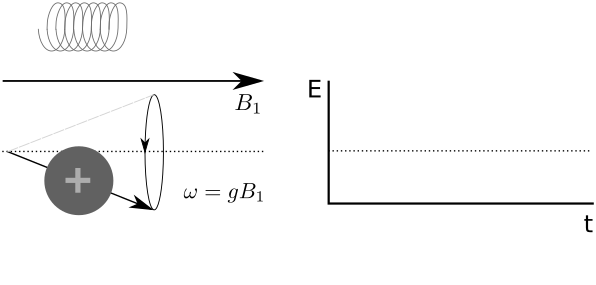
\includegraphics[width=\textwidth]{3.mri/img/spin0.png}
    \caption{Spin under a weak electromagnetic field. The precessing happens close to the magnetic fields direction and the coil does not detect it.}
    \label{fig:nosignal}
\end{minipage} ~ %add desired spacing between images, e. g. ~, \quad, \qquad, \hfill etc. %(or a blank line to force the subfigure onto a new line) 
\hfill
\begin{minipage}[b]{0.49\textwidth}
    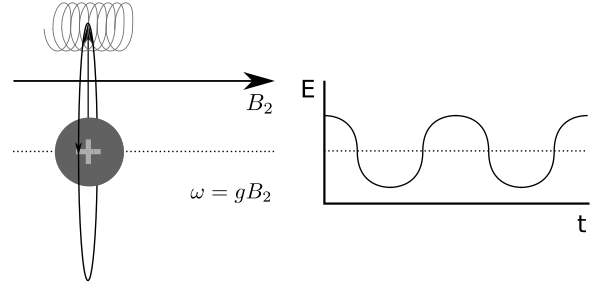
\includegraphics[width=\textwidth]{3.mri/img/spin1.png}
    \caption{After increasing the electromagnetic field, the precessing starts to move to the transversal plane, and the coil detects it.}
    \label{fig:signal}    
\end{minipage} ~ %add desired spacing between images, e. g. ~, \quad, \qquad, \hfill etc. %(or a blank line to force the subfigure onto a new line) 

\end{figure*}

\subsection{Magnetic Resonance Imaging Scanner}

A MR scanner is a machine able to create strong magnetic fields and radio frequency pulses in different frequencies.
Particularly, while functioning a MR is constantly emiting an homogeneus magnetic field refered as $B_0$ (Fig. \ref{fig:unif}).
In order to obtain the relaxation time of a particular point in the body it uses gradient magnetic fields.
A gradient is a magnetic field which strenght varies linearly along a specific direction.
When a gradient is applied, all the protons along its direction vary their Larmor frequency in a predictable way.
By applying a gradient $G_z$ in the $z$ direction (Fig \ref{fig:grad}), the angular velocity of a proton respect to its position will be:

$$\omega(z) = B_z(z) g$$.

This ensures us that if we apply a radio frequency (RF) pulse with a frequency of $B_z(z_o) g$, only the protons in the position $z_0$ will resonate.
Therefore, the signal obtained by the coil will only correspond to the protons in the slice at position $z_0$.
It's important to state that, because of hardware limitations, it's imposible to generate a RF pulse in an exact frequency.
What actually happens is that the pulse is generated for a small slice of frequencies, meaning that the protons in a small band around $z_0$ will also resonate (Fig. X).
This process is known as slice selection.

\begin{figure*}[h!]
\begin{minipage}[b]{0.49\textwidth}
    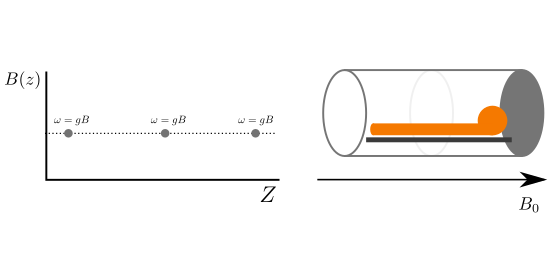
\includegraphics[width=\textwidth]{3.mri/img/grad0.png}
    \caption{\small  When protons a set of protons is placed inside an uniform magnetic field, they will all start to precess at the same velocity.}
     \label{fig:unif}
\end{minipage} ~
\hfill
\begin{minipage}[b]{0.49\textwidth}
    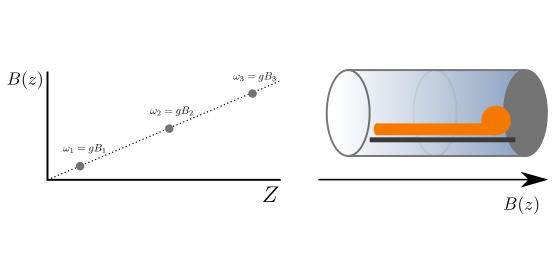
\includegraphics[width=\textwidth]{3.mri/img/grad1.png}
    \caption{\small If a linear gradient magnetic field is applied, the velocity at which the protons precess will variate in a predictable way.}
    \label{fig:grad}
\end{minipage} ~

\end{figure*}

Once the desired slice is selected, we still need to apply two more gradients in order to recover the intensities at each point of the slide.
So far, all of the protons inside of the slice are precessing in the same way.
We can think of the slice as a two dimentional matrix, with two coordinates: $x$ being the columns and $y$ being the rows.
The first gradient is applied for a short period of time in one of the directions, lets say $y$.
After the gradient is shutted down, the protons in each row will return to the same precessing velocity, but they'll have a different phase [FIG].
If then we apply a new gradient in the $x$ direction, now it will happen that:
the protons of each row will be oscilating in a different face,
and the protons of each column will be oscilating at a different velocity.
This means that, in our matrix, our information is encoded by phase in the rows and by velocity in the columns [FIG].
But when we take signal, we take signal for the whole column.
We need to repeat this for different strenghts of phase gradient $Gx$.
Now we have a bunch of signals, that come from different frequencies (columns) and different strenghts in the Gx, with greater and greater relative changes in phase.
This is called k-space [REF] ($https://www.youtube.com/watch?v=wux9L8892KE$).
Then you need to do a 2D fourier transform to recover the image.

\begin{figure*}[h!]
                                                                                                                        
\begin{minipage}[b]{\textwidth}
    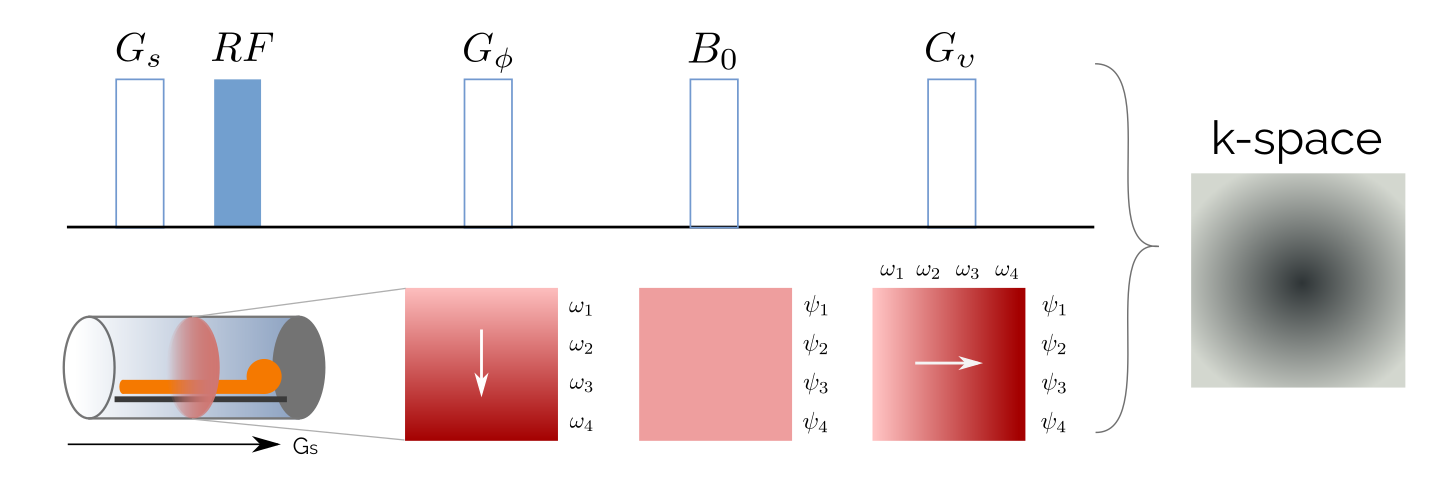
\includegraphics[width=\textwidth]{3.mri/img/kspace.png}
    \caption{Pipeline of a Magnetic Resonance adquisition.}
    \label{fig:kspace}
\end{minipage} ~

\end{figure*}

%In 1946, Bloch \cite{Bloch1946} shows that the variation in Magnetization over time is expressed as:

%$$ \frac{dM(t)}{dt} = \gamma M(t) \times B(t) 
%                      - \frac{M(t) \vec{x} + M(t)\vec{y}}{T_2}
%                      - \frac{(M(t)-M(0))\vec{z}}{T1} $$

%Where $\gamma$ is the gyromagnetic ratio, $B$ is the magnetic field intensity and T1, T2 are relaxation times.

\section{Diffusion Magnetic Resonance Imaging}
The molecules inside a fluid in equilibrium are not still, on the contrary, they are randomly moving around.
This physical phonomena is known as diffusion.
Implications of diffusion in medicine.

In 1956, H.C. Torrey \cite{Torrey1956} observes that the magnetization can be lost by effect of diffusion.
Somebody comes with a new idea of how to measure diffusion by introducing two new gradients.
Let's explain the process in a intuitive way.

Imagine that after applying the RF pulse to do slice selection, we add a gradient field $G_1=G_d$ for a small time $\delta$ms.
As explained in the previous section (sec. X), this will make the protons be off-phase between them.
If after a $\Delta$ time we apply the same gradient, but in the opossite direction $G_2=-G_d$, also for $\delta$ms, then, the protons should go back to be in-phase [fig].
However, the particules undergoing diffusion will have moved (fig.), for which the second gradient $G_2$ would have reach them in a different place, and therefore, change their angular velocity differently.
In this way, a difference in the phase of the protons respect to the rest is a sign of diffusion [fig].
Since a voxel now has protons precessing at different velocities, they create less signal.
Max. signal is achieved when they all rotate together.
The difference between the signal obtained with no diff. gradient and with diff. gradient reflects the amount of diffusion.


\begin{figure}
    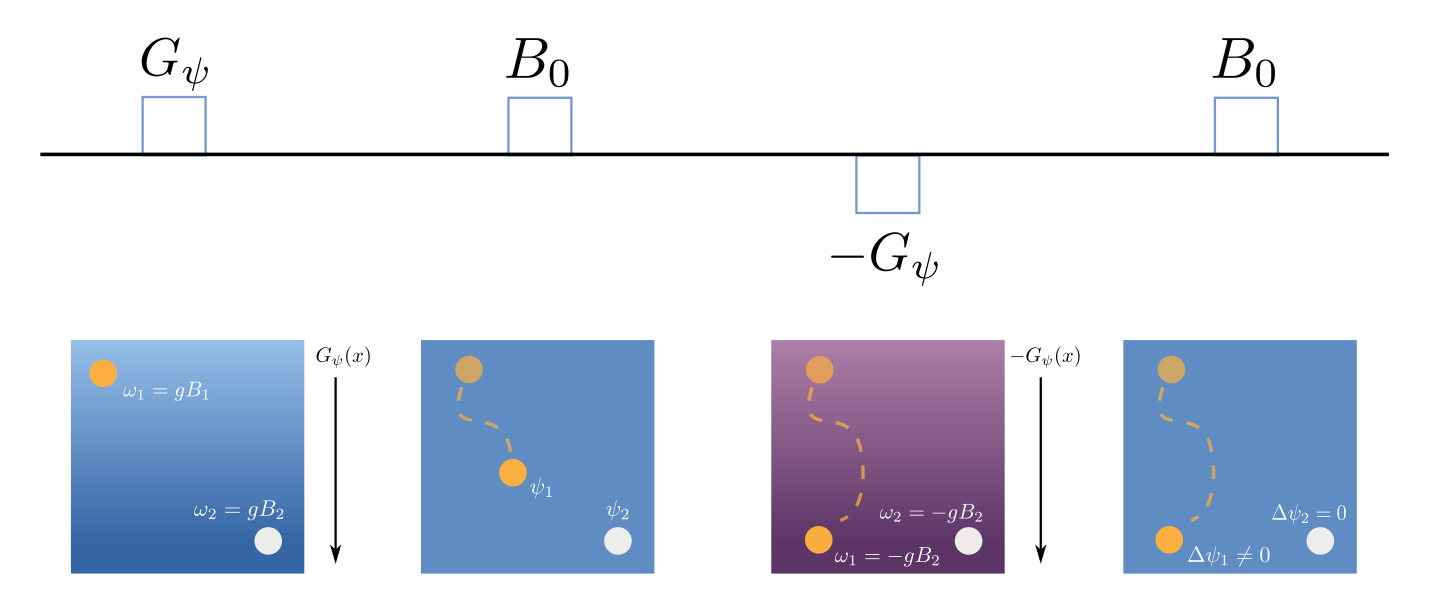
\includegraphics[width=0.49\textwidth]{3.mri/img/dmri.png}
    \caption{Figure explaining dMRI}
    \label{fig:}
\end{figure}  

\subsection{Pulsed Gradient Spin Echo (PGSE)}
\begin{figure}
    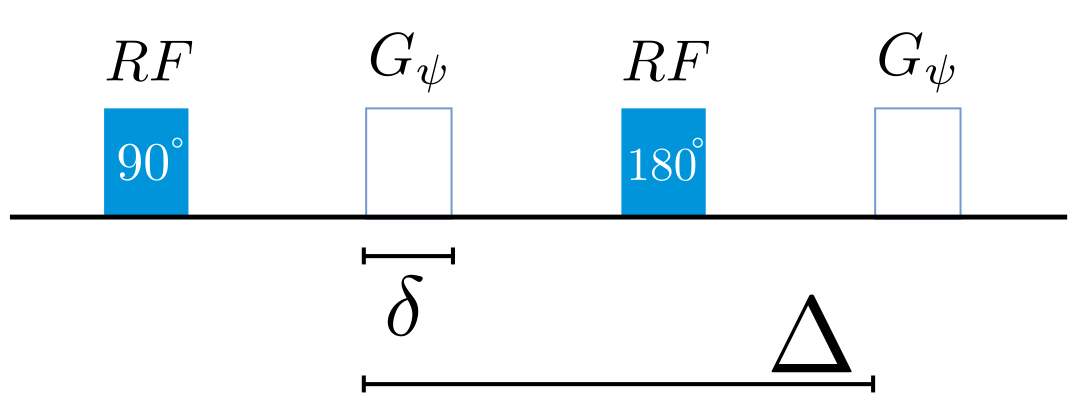
\includegraphics[width=0.49\textwidth]{3.mri/img/fgp.png}
    \caption{Secuencia Pulsed Gradient Spin Echo.}
    \label{fig:fgp}
\end{figure}  

[refrase all]
In 1965, Stejskal and Tanner invent the PGSE sequence to measure diffusion. 
The Stejskal-Tanner imaging sequence [Stejskal and Tanner (1965)] is used to
measure the diffusion of water molecules in a given direction. This pulse
sequence is illustrated in Figure 4.3. This sequence uses two gradient pulses
in the direction g, of duration time δ, to control the diffusion-weighting.
They are placed before and after a 180◦ degrees refocusing pulse.
More specifically, a first 90◦ degrees RF is applied to flip the magnetization
in the transverse plane. The first gradient pulse causes a phase shift of the
spins whose position are now a function of time. Spin position is in fact
assumed to stay constant during time δ. Finally, the 180◦ pulse combined with
the second gradient pulse induces another phase shift. It is applied after a time
∆ separating the two gradient pulses. This pulse cancels the first phase
shift only for static spins. On the other hand, spins under Brownian motion during
the time period ∆ separating the two pulses undergo different phase shifts by
the two gradient pulses, resulting in a T2 signal attenuation [Cercignani and Horsfield. (2001)].
By assuming the pulses to be infinitely narrow (narrow pulse approximation), i.e.
if the gradient pulse duration δ is short enough for the diffusion of the water molecule
to be negligible during that time, [Stejskal and Tanner (1965)] showed that the signal
attenuation S(q,τ) is expressed as the 3-dimensional (3D) Fourier transform
F of the ensemble average propagator P,

[some eq?]

where $E(g, \delta, \Delta)$;
$g$ is the intensity of the gradient field;
$S_0$ is the signal obtained with no diffusion gradient ($g=0 T/m$)
, and $\gamma$ is the gyromagnetic ratio of water.
Notice that we need $S_0$ in the equation, since the diffusion comes from the difference in signal between the 

Assuming the pdf to be gaussian, we get:

\begin{equation}
    E(g, \delta, \Delta) = 
    \frac{S(g, \delta, \Delta)}{S_0} =
         e^{-\gamma^2 g^2 \delta^2 \left(\Delta - \frac{\delta}{3}\right) D} 
    \label{eq:st}
\end{equation}

\subsection{subsection}
In 1985 Le Bihan \cite{LEBIHAN} proposses to gather all the parameters in a single one: 

$$ b = \gamma^2 g^2 \delta^2 \left(\Delta - \frac{\delta}{3}\right) $$ ,

simplifiying the equation \ref{eq:st} to:

$$ E(b) = \frac{S(b)}{S_0} = e^{-b D} $$

where $b$ represents the reciprocal of the diffusion intensity.

In 1994 Basser et al. \cite{Basser1994} propose to measure the signal atenuation in different directions, and then approximate the diffusion coefficient with a second order tensor.
A tensor is a multidimentional matrix associated to a base, which possess a transformation law indicating how the tensor components change when the base change.
This sets the bases of what's known as DTI.
DTI represents the diffusion as a 3-dimentional (3D) elipsoide, which can be coded in a symmetric matrix:

$$
    D =
    \begin{pmatrix}
             D_{xx} & D_{xy} & D_{xz} \\
             D_{xy} & D_{yy} & D_{yz} \\
             D_{xz} & D_{yz} & D_{zz}    
    \end{pmatrix}
$$

Therefore we need at least 6 acquisitions.

One of the main limitants of this method is that it does not allow to
represent the crossing of fibers. They get modeled as spheres.

In 1991 Callaghan et al. \cite{Callaghan1991} developped the q-space analysis.
This allows to make microscopy with dMRI.
Based on the work of Stejskal and Tanner, Callaghan show that it's possible to express the signal attenuation as:

$$E(q,\Delta) =  \frac{S(q,\Delta)}{S_0} = \int_{R^2}{p(r;\Delta)e^{-2\pi i q r} dr} $$
$$ q = \frac{\gamma \delta g}{2\pi} $$

Where $p(r;t)$  is the probability density that a set of particles travels a distance $r$ during a time $t$.
Because of this, $p(r;t)$ is highly related to the compartment where the particles are contained.

One of the main advantages of q-space over DTI is that is does not assume any a prior model, allowing to define different strategies for $p(r;t)$.
Here we talk about \textit{Spherical Harmonics} \cite{Tuch2004} and
\textit{Constrained Spherical Deconvolution} \cite{Tournier2004}, which are the most relevant ones for this thesis.

\section{Tractography}

%TODO
% Explain tractography as a random walk
% Explain its problems
%  Gyral bias
%  Resolution
%  No direction (Jbabdi and Beherens)
%  False positives!!!!!
% Explains that anyway it's the best thing we have

Diffusion in the white matter is constrained by the tracts present on it.
The protons present in any point of the brain will be able to diffuse only inside a tract and along its path.
This means that, by following the diffusion signal, we should be able to trace the brain pathways.
However, most of the methods to model diffusion signal cannot handle correctly the crossing of fibers.
The best we can do, is to derive a probabilistic map from one voxel to another, and simulate the random movement of a water particle from one voxel to another.
We hope that the diffusion signal + some constraints in the random walk allow us to retrieve the real pathways of the brain.
Furthermore, if we generate a big number of this random walks, or streamlines, we hope to be able to recover the underlying tracts in a correct way by means of statistics.
They are some issues with this.
But there are some cool stuff about it also.

[VAN ESSEN]
Using high-resolution postmortem diffusion imaging and tractography in Old World monkeys, we found a correlation coefficient of ~0.58 between tractography-based and tracer- based estimates of connectivity;
the correlation is highest for strong, short-distance pathways but is informative even for weak connections and widely separated areas (Donahue et al., 2016).
We will discuss multiple reasons why tractography imperfectly reflects ground-truth neuroanatomical connectivity.
This includes
(i) a gyral bias in which tractography streamline within ‘gyral blades’ are biased towards gyral crowns rather than sulcal banks (Van Essen et al., 2014);
(ii) an ‘anti-fundus’ bias in which connections to/from sulcal fundi tend to be obscured by tangential fiber bundles immediately subjacent to many sulci (Reveley et al., 2015);
(iii) axonal branching within white matter that includes many branches at approximately right angles (Economo et al., 2016) that are inherently difficult to discriminate from crossing fibers that also occur within white matter;
and (iv) potential dispersion or ‘defasciculation’ in the white matter axonal trajectories of pathways that interconnect widely separated gray matter parcels (Jbabdi et al., 2015).


[MINE]
A primary issue is the spatial resolution of diffusion imaging:
it is several orders of magnitude coarser than axonal diameters (millimeters vs. micrometers) (Van Essen et al., 2014), making hard to infer some brain pathways.
In addition, there is as yet no quantitative measure of the strength of connections from diffusion (Jbabdi and Behrens, 2013).
Given a seed-point in the brain, prob- abilistic tractography creates a tractogram:
an image where each voxel is valued with its probability of being connected to the seed through axonal bundles.
One way of calculating these probabilities is with a Monte Carlo procedure, simulating the random walk of water particles through the white matter (Behrens et al., 2003).
Each one of these paths is known as a streamline.

[MAXIME NATURE NEUROSCIENCE?]
we organized an open international tractography challenge, which resulted in 96 distinct submissions from 20 research groups.
To determine the current state of the art in tractography, we organized  an  international tractography competition and employed a novel validation method based on simulated DWI of a brain‐like geometry.
This ground truth data set represented 25 well‐known valid bundles that covered approximately 70\% of the human brain white matter.

While most state‐of‐the‐art algorithms  reconstructed 90\% of ground truth bundles to at least some extent, on average they produced four times more invalid than valid  bundles. About half of the invalid bundles occurred systematically in the majority of submissions. 
The average ratio of false‐positive to true‐positive bundles was approximately four to one.
This ratio could not be improved by employing higher quality data or even using the gold standard field of local orientations, highlighting that current tractography approaches are fundamentally ill‐posed.


\section{fMRI}
\cite{Glover2011}
All the processes of neural signaling in the brain require energy in the form of adenosine triphosphate (ATP).
When a region of the brain is up-regulated (i.e. activated) by a cognitive task such as finger tapping, the additional neural firing and other increased signaling processes result in a locally increased energy requirement.
The brain respondes by adjusting its blood flow to deliver nutrients such as oxygen and glucose to stressed tissues and allow them to function. Haemodynamic response (HR) allows the rapid delivery of blood to active neuronal tissues.
The second mechanism, termed Blood Oxygenation Level Dependent (BOLD) contrast, was first demonstrated in rats48,50 and later in humans3,37,49,52, and is the contrast that is used in virtually all conventional fMRI experiments. BOLD contrast results from the change in magnetic field surrounding the red blood cells depending on the oxygen state of the hemoglobin. When fully oxygenated, HbO2 is diamagnetic and is magnetically indistinguishable from brain tissue. However, fully deoxygenated Hb has 4 unpaired electrons and is highly paramagnetic59. This paramagnetism results in local gradients in magnetic field whose strength depends on the [Hb] concentration. These endogenous gradients in turn modulate the intra- and extra-vascular blood’s T2 and T2* relaxation times through diffusion and intravoxel dephasing, respectively. Using a gradient refocused echo (GRE) MRI pulse sequence7, the acquisition is made sensitive to T2* and T2. At 1.5T and
3T, the T2* contrast is predominant and is largest in venules61, while at higher field strength the diffusion-weighted contrast of T2 relaxation becomes more important and, because signals are generated preferentially in capillaries and tissue with spin-echo acquisitions, provides greater spatial specificity57,64. Since most fMRI is currently performed at 3 Tesla or below, BOLD fMRI utilizes primarily GRE methods because of the increased T2* contrast10.

[wikipedia et al.]
Cerebral blood flow (CBF) is the blood supply to the brain in a given period of time.[     Tolias C and Sgouros S. 2006. "Initial Evaluation and Management of CNS Injury."]
The most common functional imaging signal is the blood-oxygen-level dependent signal (BOLD), which primarily corresponds to the concentration of deoxyhemoglobin.[12] The BOLD effect is based on the fact that when neuronal activity is increased in one part of the brain, there is also an increased amount of cerebral blood flow to that area which is the basis of haemodynamic response. This increase in blood flow produces an increase in the ratio of oxygenated hemoglobin relative to deoxygenated hemoglobin in that specific area. The difference in magnetic properties of oxygenated and deoxygenated hemoglobin is what allows fMRI imaging to produce an effective map of which neurons are active and which are not. In short, deoxygenated hemoglobin is paramagnetic while oxygenated hemoglobin is diamagnetic. Diamagnetic blood (oxyhemoglobin) interferes with the magnetic resonance (MR) signal less and this leads to an improved MR signal in that area of increased neuronal activity. However, Paramagnetic blood (deoxyhemoglobin) makes the local magnetic field inhomogenous. This has the effect of dephasing the signal emitted in this domain, causing destructive interference in the observed MR signal. Therefore, greater amounts of deoxyhemoglobin lead to less signal. Neuronal activity ultimately leads to an increase in local MR signaling corresponding to a decrease in the concentration of deoxyhemoglobin.[13]
